\documentclass{article}
\usepackage[utf8]{inputenc}
\usepackage{graphicx}
\usepackage{ragged2e}
\usepackage[margin=2.5cm]{geometry}
\usepackage{array}
\usepackage{wrapfig}
\usepackage{multirow}
\usepackage{tabularx}
\usepackage{amsmath}
\usepackage{wrapfig}
\usepackage{mathtools}
\usepackage[table]{xcolor}
\usepackage{multirow}
\usepackage{polski}
\usepackage{rotating}
\title{Charakterystyki statyczne pomieszczenia z grzejnikiem.}

\author{Jan Bronicki 249011\\
Marcin Gruchała 248982\\}
\date{}

\begin{document}
\maketitle

\section{Cel ćwiczenia.}
Stworzenie charakterystyki statycznej, dla pomieszczenia z grzejnikiem.
\section{Wstęp.}
Opisujemy model pomiesczenia z grzejnikiem. Model jest uproszczonym matematycznym opisem jakiegoś obiektu. Przy opisie pomieszczenia naszym modelem będzie bilans ciepła, dla tego pomieszczenia, ponieważ naszym celem jest wyznaczenie współczynników strat ciepła oraz stworzenie charkterystyk statycznych opisujących temperature w pomieszczeniu. Poniższy rysunek przedstawia model opisujący nasz badany obiekt.
\begin{figure}[h]
    \centering
    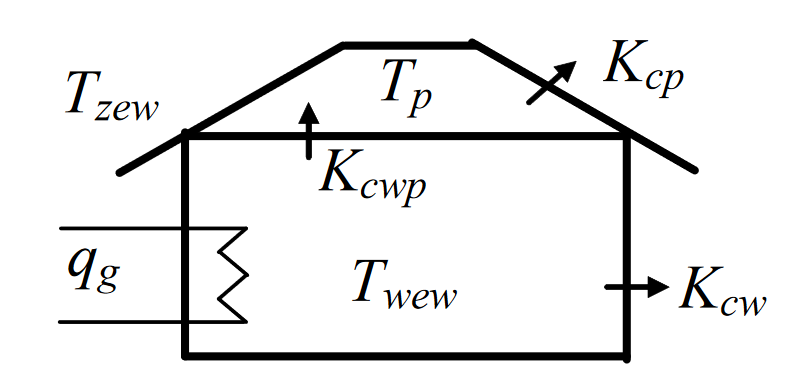
\includegraphics[width=0.5\textwidth]{dom.png}
    \label{fig:my_label}
\end{figure}
$\\
\text{Gdzie:}\\
T_{zew} - \text{temperatura\ na\ zewnątrz\ pomieszczenia}\\
T_{wew} - \text{temperatura\ wewnątrz\ pomieszczenia} \\
T_{p} - \text{temperatura\ na\ poddaszu}\\
Q_g - \text{grzejnik}\\
K_{cw} - \text{współczynnik\ strat\ ciepła\ przez\ ściany} \\
K_{cwp} - \text{współczynnik\ strat\ ciepła\ przez\ sufit} \\
K_{cp} - \text{współczynnik\ strat\ ciepła\ przez\ dach}\\
$
\begin{flushleft}
Poniższy układ równań przedstawia bilans ciepła, dla pomieszczenia.
\end{flushleft}
$$
 \begin{cases}
        0=Q_{g} -K_{cw} (T_{wew} - T_{zew})-K_{cwp} (T_{wew} -T_{p})\\
        0=K_{cwp}(T_{wew}-T_{p})-K_{cp}(T_{p}-T_{zew})
\end{cases}
$$
Dla powyższych równań znamy:
\begin{flushleft}
    $Q_{g}=1000W$ \\
    $T_{zew}=-20^{\circ}C$\\
    $T_{wew}=20^{\circ}C$\\
    $T_{p}=10^{\circ}C$\\
    $\alpha=0,25$\\
    $K_{cwp}=\alpha K_{cw} \implies K_{cwp}=0,25K_{cw}$\\
\end{flushleft}


\newpage
\begin{flushleft}
\section{Rozwiązanie układów rwónań ze względu na $K_{cp}, K_{cwp}, K_{cw}$ oraz $T_{wew}, T_{p}$(tradycyjnie).}

\end{flushleft}
$$
 \begin{cases}
        0=Q_{g} -K_{cw} (T_{wew} - T_{zew})-K_{cwp} (T_{wew} -T_{p})\\
        0=K_{cwp}(T_{wew}-T_{p})-K_{cp}(T_{p}-T_{zew})
\end{cases}
$$

\begin{center}
     $Q_{g}=1000W$ \\
    $T_{zew}=-20^{\circ}C$\\
    $T_{wew}=20^{\circ}C$\\
    $T_{p}=10^{\circ}C$\\
    $\alpha=0,25$\\
    $K_{cwp}=\alpha K_{cw} \implies K_{cwp}=0,25K_{cw}$\\
\end{center}


Ze względu na $K_{cp}, K_{cwp}, K_{cw}$:
\begin{center}
    $
    \begin{cases}
        K_{cw}T_{wew}-K_{cw}T_{zew}+0,25K_{cw}T_{zew}-0,25K_{cw}T_{p}=Q_{g}\\
        0,25K_{cw}T_{wew}-0,25K_{cw}T_{p}-K_{cp}T_{p}+K_{cp}T_{zew}=0
    \end{cases}
    $
    
    $
    \begin{cases}
        K_{cw}(1,25T_{wew}-0,25T_{p}-T_{zew})=Q_{q}\\
        K_{cp}(T_{p}-T_{zew})-0,25K_{cw}(T_{wew}-T_{p})=0
    \end{cases}
    $
    \vspace{1ex}
    \\
    $
    K_{cp}=\frac{0,25K_{cw}(T_{wew}-T_{p})}{T_{p}-T_{zew}}
    $
    \\
    \vspace{1ex}
    $
    K_{cw}=\frac{Q_{g}}{0,75T_{wew}-T_{zew}-0,25T_{p}}
    $
    \\
    \vspace{1ex}
    $
    K_{cw}=\frac{1000}{25-2,5+20}\approx 23,53
    $
    \\
    \vspace{1ex}
    $
    K_{cp}=\frac{0,25 \cdot 23,53(20-10)}{10-(-20)}\approx1,96
    $
    \\
    \vspace{1ex}
    $
    K_{cwp}=0,25K_{cw}\approx 5,98
    $
\end{center}

Ze względu na  $T_{wew}, T_{p}$:
\begin{center}
    $
    \begin{cases}
        T_{wew}=\frac{Q_{g}+K_{cw}T_{zew}+0,25T_{p}K_{cw}}{1,25K_{cw}}\\
        T_{p}=\frac{0,2Q_{g}+0,2T_{zew}K_{cw}+T_{zew}K_{cw}}{0,2K_{cw}+K_{cp}}
    \end{cases}
    $
    \\
    \vspace{1ex}
    $
    \begin{cases}
        T_{wew}=\frac{Q_{g}+K_{cw}T_{zew}+0,25K_{cw}\frac{0,2Q_{g}+0,2T_{zew}K_{cw}+T_{zew}K_{cw}}{0,2K_{cw}+K_{cp}}}{1,25K_{cw}}\\
        T_{p}=\frac{0,2Q_{g}+0,2T_{zew}K_{cw}+T_{zew}K_{cw}}{0,2K_{cw}+K_{cp}}
    \end{cases}
    $
    \\
    \vspace{1ex}
   
    $
    T_{wew}=\frac{1000+23,53\cdot(-20)+0,25\cdot23,53\frac{0,2\cdot1000+0,2\cdot(-20)\cdot23,53+(-20)\cdot1,96}{0,2\cdot23,53+1,96}}{1,25\cdot23,53} \approx 20
    $\\
     \vspace{1ex}
    $
    T_{p}=\frac{0,2\cdot1000+0,2\cdot(-20)\cdot23,53+(-20)\cdot1,96}{0,2\cdot23,53+1,96} \approx 10
    $
\end{center}

\begin{flushleft}
\section{Rozwiązanie układów rwónań ze względu na $K_{cp}, K_{cwp}, K_{cw}$ oraz $T_{wew}, T_{p}$(macierzowo).}
\end{flushleft}

\begin{flushleft}
Ze względu na $K_{cp}. K_{cwp}, K_{cw}$:
\end{flushleft}
$$
\begin{bmatrix}
        0 & 1,25T_{wew}-0,25T_{p}-T_{zew}            \\[0.3em]
        T_{p}-T_{zew} & -0,25(T_{wew}-T_{p})            \\[0.3em]
    \end{bmatrix}
    \begin{bmatrix}
        K_{cp}\\
        K_{cw}
    \end{bmatrix}
    =
    \begin{bmatrix}
        Q_{q}\\
        0
    \end{bmatrix}
$$

$$
W=
\begin{bmatrix}
        0 & 1,25T_{wew}-0,25T_{p}-T_{zew}            \\[0.3em]
        T_{p}-T_{zew} & -0,25(T_{wew}-T_{p})            \\[0.3em]
    \end{bmatrix}
$$
$$
K=
\begin{bmatrix}
        K_{cp}\\
        K_{cw}
    \end{bmatrix}
$$

$$
Y=\begin{bmatrix}
        Q_{q}\\
        0
    \end{bmatrix}
$$

$$
WK=Y
$$

$$
K=W^{-1}Y=
\begin{bmatrix}
        1,960784313725490\\
        23,529411764705880
\end{bmatrix}\approx 
\begin{bmatrix}
        1,96 \\
        23,53
\end{bmatrix}
$$

\begin{flushleft}
Ze względu na  $T_{wew}, T_{p}$:
\end{flushleft}

$$
\begin{bmatrix}
        (K_{cw}+0,25K_{cw})& -(0,25K_{cw})            \\[0.3em]
        0,25K_{cw} & (0,25K_{cw}-K_{cp})            \\[0.3em]
    \end{bmatrix}
    \begin{bmatrix}
        T_{wew}\\
        T_{p}
    \end{bmatrix}
    =
    \begin{bmatrix}
        Q_{q}+K_{cw}T_{zew}\\
        -K_{cp}T_{zew}
    \end{bmatrix}
$$

$$
O=\begin{bmatrix}
        (K_{cw}+0,25K_{cw})& -(0,25K_{cw})            \\[0.3em]
        0,25K_{cw} & (0,25K_{cw}-K_{cp})            \\[0.3em]
    \end{bmatrix}
$$

$$
T=\begin{bmatrix}
        T_{wew}\\
        T_{p}
    \end{bmatrix}
$$

$$
P=\begin{bmatrix}
        Q_{q}+K_{cw}T_{zew}\\
        -K_{cp}T_{zew}
    \end{bmatrix}
$$

$$
OT=P
$$

$$
T=O^{-1}P=
\begin{bmatrix}
       20 \\
       10
\end{bmatrix}
$$

\begin{flushleft}
Macierze obliczyliśmy w programie Matlab.
\end{flushleft}


\section{Wykresy.}
Wykresy wygenerowaliśmy w programie Matlab, znajdują się na następnej stronie sprawozdania.

\begin{figure}
    \centering
    \begin{turn}{270}
    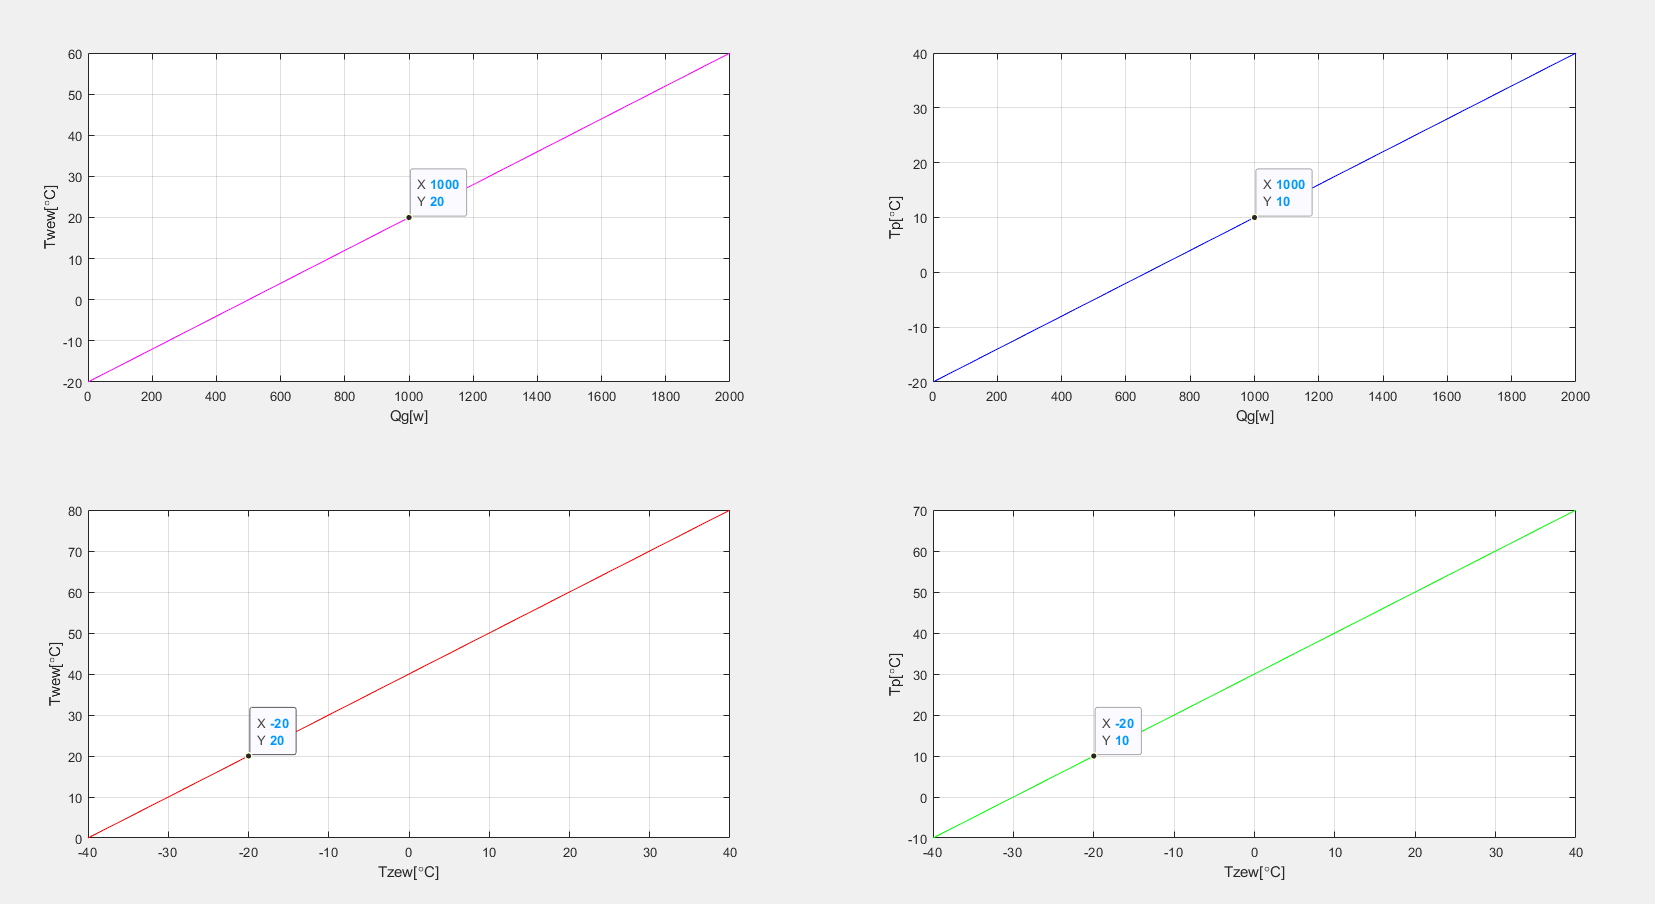
\includegraphics[width=1.5\textwidth]{Dom_wykresy.png}
    \end{turn}
    \label{fig:my_label}
\end{figure}

\section{Wnioski.}
Jak widać tworzenie modeli oraz charakterystyk statycznych bywa bardzo pomocnę ponieważ pozwala lepiej zrozumieć i przewidzieć zmiany zachodzące w badanym obiekcie. W czytelny sposób przedstawia zachowanie się obiektu w zależności od różnych parametrów.  
\begin{figure}
    \centering
    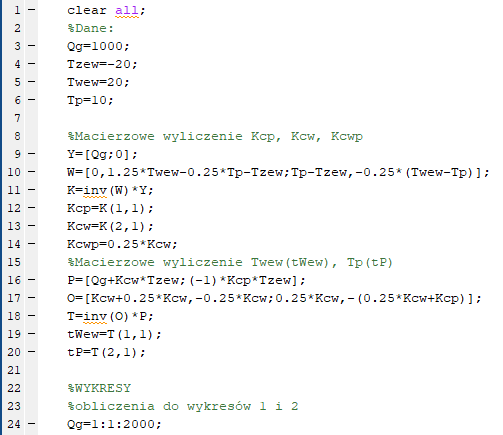
\includegraphics[width=0.8\textwidth]{kod1.png}
    \label{fig:my_label}
\end{figure}

\begin{figure}
    \centering
    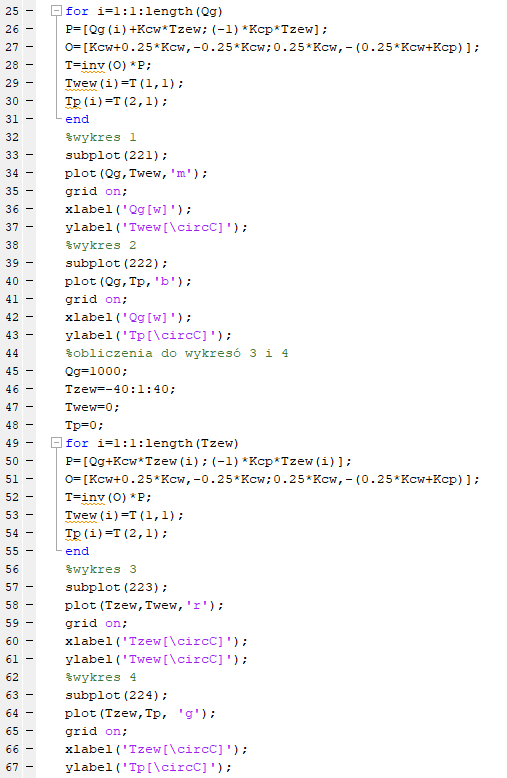
\includegraphics{kod2.png}
    \label{fig:my_label}
\end{figure}
\end{document}






